\section{Sistemas de alarma sísmica}
Es un sistema de sensores sísmicos distribuidos en el centro y la costa oeste de México, diseñado para detectar movimientos sísmicos y emitir alertas tempranas a fin de advertir a las autoridades de protección civil y a la sociedad en general cuando ocurra un sismo que pueda afectar a ciudades vulnerables.
La alarma se activa con sismos de magnitudes cercanas a los 6 grados y se transmite en los 8 mil 200 altavoces distribuidos en las 16 delegaciones de la Ciudad de México. 
Es un sistema que genera una alerta con un tiempo de oportunidad previo al arribo de un sismo de sismos fuertes generados en las zonas sísmicas de mayor peligro para la población vulnerable, con el objetivo de contribuir a mitigar los posibles efectos. 
\begin{figure}[htbp]
	\begin{center}
		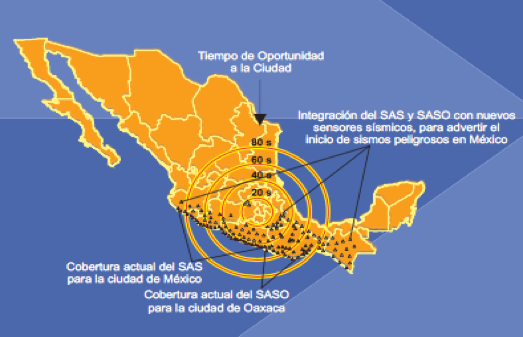
\includegraphics[width=.4\textwidth]{images/imgmarco/mapa2}
		\label{fig:mapa2}
	\end{center}
\end{figure}


\section{Transmisión de alarma sísmica}
El sistema se basa en el principio de las ondas sísmicas superficiales, las cuales son consideradas como potencialmente dañinas; éstas viajan de entre 3.5 y 4.0 kilómetros por segundo, lo que significa que tardan entre 75 y 85 segundos en viajar de Guerrero a la Ciudad de México.\\Oficialmente, la alarma se activa con sismos de magnitudes cercanas a los 6 grados y se transmite en los 8 mil 200 altavoces distribuidos en las 16 delegaciones de la Ciudad de México. \\
Para la ciudad de México es 162.450 MHz (canal 3), 162.500 MHz (canal 5) y 162.550 MHz (canal 7).
Para Acapulco y Oaxaca 162.400 MHz (canal 1).
Y Chilpancingo 162.425 MHz (canal 2).\\Los canales son para los radios de frecuencia familiar con NOAA(La Administración Nacional Oceánica y Atmosférica).
\begin{figure}[htbp]
	\begin{center}
		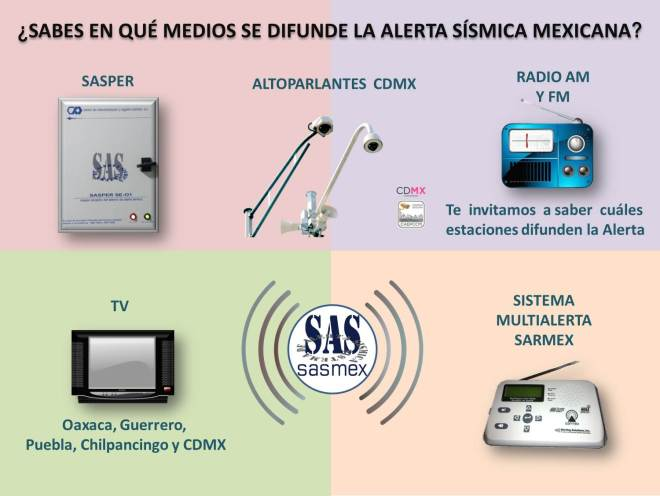
\includegraphics[width=.4\textwidth]{images/imgmarco/transmision}
		\label{fig:transmision}
	\end{center}
\end{figure}

\section{Sistema de información georeferenciado}
Un Sistema de Información Georeferenciada (GIS) es una integración organizada de hardware, software y datos geográficos diseñado para capturar, almacenar, manipular, analizar y desplegar en todas sus formas la información geográficamente referenciada con el fin de resolver problemas complejos de planificación y gestión. También puede definirse como un modelo de una parte de la realidad referido a un sistema de coordenadas terrestre y construido para satisfacer unas necesidades concretas de información.

Los SIG nos permiten hacer un análisis exhaustivo del territorio en los ámbitos más diversos. Son herramientas versátiles, con un amplio campo de aplicación en cualquier actividad que conlleve un componente espacial.
Así, la tecnología de los Sistemas de Información Geográfica puede ser utilizada para investigaciones científicas, para gestión de los recursos y activos, en arqueología, en evaluación del impacto ambiental, para la planificación urbana, en cartografía, sociología, geografía histórica, marketing o logística, por nombrar sólo algunos ámbitos de aplicación.

El SIG funciona como una base de datos con información geográfica (datos alfanuméricos) que se encuentra asociada por un identificador común a los objetos gráficos de un mapa digital. De esta forma, señalando un objeto se conocen sus atributos e, inversamente, preguntando por un registro de la base de datos se puede saber su localización en la cartografía.
La razón fundamental para utilizar un SIG es la gestión de información espacial. El sistema permite separar la información en diferentes capas temáticas y las almacena independientemente, permitiendo trabajar con ellas de manera rápida y sencilla, facilitando al profesional la posibilidad de relacionar la información existente a través de la topología de los objetos, con el fin de generar otra nueva que no podríamos obtener de otra forma.
Las principales cuestiones que puede resolver un Sistema de Información Geográfica, ordenadas de menor a mayor complejidad, son:
\begin{enumerate}
\item Localización: preguntar por las características de un lugar concreto.
\item Condición: el cumplimiento o no de unas condiciones impuestas al sistema.
\item Tendencia: comparación entre situaciones temporales o espaciales distintas de alguna característica.
\item Rutas: cálculo de rutas óptimas entre dos o más puntos.
\item Pautas: detección de pautas espaciales.
\item Modelos: generación de modelos a partir de fenómenos o actuaciones simuladas.
\end{enumerate}

\begin{figure}[htbp]
	\begin{center}
		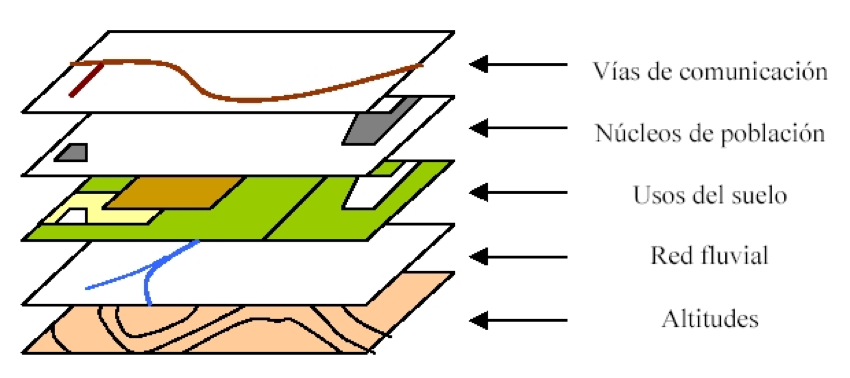
\includegraphics[width=.4\textwidth]{images/imgmarco/sistemageo}
		\label{fig:sistemageo}
	\end{center}
\end{figure}

\section{Diferencia entre Geolocalización y Georeferenciación}
Algunas de las funciones más utilizadas por los usuarios pueden ser: cómo llegar a un lugar utilizando el trayecto más corto, ubicar en el mapa nuestro próximo destino de vacaciones, o informar a algún familiar de exactamente el lugar en el que nos encontramos. A la hora de utilizar estos servicios, aparecen dos conceptos: la geolocalización y la georreferenciación.
Aunque a priori puedan parecer lo mismo, y de hecho en muchas ocasiones se utilicen indistintamente, existen varias diferencias entre los mismos, tanto en su definición como en sus aplicaciones y es importante conocerlas para poder hablar con propiedad. La georreferenciación se define como un proceso por el cual se dota de un sistema de referencia de coordenadas terreno a una imagen digital que originariamente se encuentra en coordenadas pixel.
Por su parte, la geolocalización se define como la identificación de la ubicación de un dispositivo por ejemplo un radar, dispositivo móvil o cualquier aparato tecnológico conectado a internet. Está relacionada con los sistemas de detección de posición, pero añade datos como información de la zona, calles, locales, etc.
Google posee dos plataformas muy conocidas por los usuarios: Google Earth y Google Maps, cada una asociada a uno de los términos. 
Google Earth es un sistema de georreferenciación que nos permite situar en el mapa puntos concretos de la geografía. Además, esta aplicación también nos permite obtener una vista aérea de las ubicaciones y navegar por ellas, pero son mapas creados a partir de la selección de un conjunto de datos.
La geolocalización por su parte tiene una característica muy específica: nos permite localizar un dispositivo en el mapa en tiempo real. Por ejemplo, lo que hace Google Maps es geolocalizar nuestro dispositivo, es decir, acceder a nuestra ubicación exacta y ofrecernos las diferentes funciones de la aplicación a partir de esto.
Es cierto que también tiene un sistema de georreferenciación, es decir, podemos ver planos de otros sitios distintos al que nos encontramos, pero la clave y valor añadido de la geolocalización es que a través de este sistema seremos capaces de localizar nuestro dispositivo y sobre todo de obtener información en tiempo real.

\section{GPS}
El sistema GPS (Sistema de Posicionamiento Global por sus siglas en inglés) hace posible determinar las coordenadas que permiten ubicar puntos específicos sobre la superficie de la Tierra. 
El GPS es un sistema de posicionamiento por satélites desarrollado por el Departamento de la Defensa de los E.U., diseñado para apoyar los requerimientos de navegación y posicionamiento precisos con fines militares. En la actualidad es una herramienta importante para aplicaciones de navegación, posicionamientos de puntos en tierra, mar y aire.
Hace ya varios años que los dispositivos telefónicos incorporan receptores de GPS. GPS o Sistema de Posicionamiento Global es una red compuesta por al menos 30 satélites que orbitan alrededor de la Tierra.
Al menos 4 de estos satélites estén visibles para nuestro dispositivo y cada satélite emite una señal sobre su ubicación cada cierto tiempo. Teniendo en cuenta la latitud, longitud, altura y tiempo se calcula la ubicación. Cuantos más satélites tomen parte en el proceso, más exacto será esta triangulación.
\begin{figure}[htbp]
	\begin{center}
		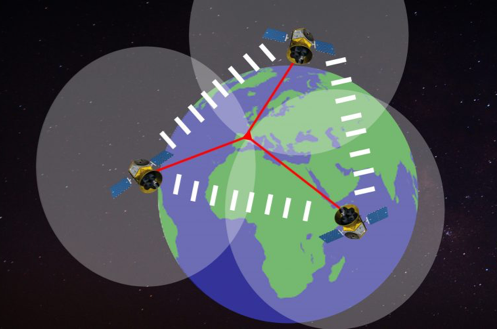
\includegraphics[width=.4\textwidth]{images/imgmarco/gps}
		\label{fig:gps}
	\end{center}
\end{figure}

\subsection{Segmento espacial}
El segmento espacial consta de una constelación de satélites que transmiten señales de radio a los usuarios.\\Los Estados Unidos mantienen la disponibilidad de no menos de 24 satélites operacionales GPS el 95% de las veces.Para garantizar este compromiso, la Fuerza Aérea ha estado volando 31 satélites GPS opercionales en los últimos años.\\
Los satélites GPS en órbita terrestreestán a una altitud media de aproximadamente 20,200 kilometros,cada satélite rodea la tierra en dos días. 
\subsubsection{2.5.1.1 Señales GPS}
Los satélites del GPS transmiten dos señales de radio de baja potencia, llamadas "L1" y "L2". Cada señal GPS contiene tres componentes de información: un código pseudoaleatorio, los datos de efemérides de satélite y datos de almanaque. El código pseudoaleatorio identifica al satélite que transmite su señal. Los datos de efemérides de satélite proporcionan información sobre la ubicación del satélite en cualquier momento. El almanaque contiene información sobre el estado del satélite y la fecha y hora actuales. Para cada satélite, el tiempo es controlado por los relojes atómicos a bordo que son cruciales para conocer su posición exacta. 


\subsubsection{2.5.1.2 Determinación de posiciones del GPS}
Aunque el GPS puede dar posiciones muy precisas, aún hay fuentes de error. Estos incluyen los errores del reloj, los retrasos atmosféricos, sin saber exactamente dónde están los satélites en sus órbitas, las señales que se refleja de los objetos en la superficie de la Tierra, e incluso la degradación intencionada de la señal del satélite. 

\subsection{Segmento de control}
Es una serie de estaciones de rastreo, distribuidas en la superficie terrestre que continuamente monitorea a cada satélite analizando las señales emitidas por estos y a su vez, actualiza los datos de los elementos y mensajes de navegación, así como las correcciones de reloj de los satélites.\\Las estaciones se ubican estratégicamente cercanas al plano ecuatorial y en todas se cuenta con receptores con relojes de muy alta precisión.
\subsection{Segmento de usuario}
Lo integran los receptores GPS que registran la señal emitida por los satélites para el cálculo de su posición tomando como base la velocidad de la luz y el tiempo de viaje de la señal, así se obtienen las pseudodistancias entre cada satélite y el receptor en un tiempo determinado, observando al menos cuatro satélites en tiempo común; el receptor calcula las coordenadas X, Y, Z y el tiempo.

\section{DGPS}
Es un sistema que proporciona a los receptores de GPS correcciones de los datos recibidos de los satélites GPS, con el fin de proporcionar una mayor precisión en la posición calculada.
El fundamento radica en el hecho de que los errores producidos por el sistema GPS afectan por igual (o de forma muy similar) a los receptores situados próximos entre sí.
\begin{figure}[htbp]
	\begin{center}
		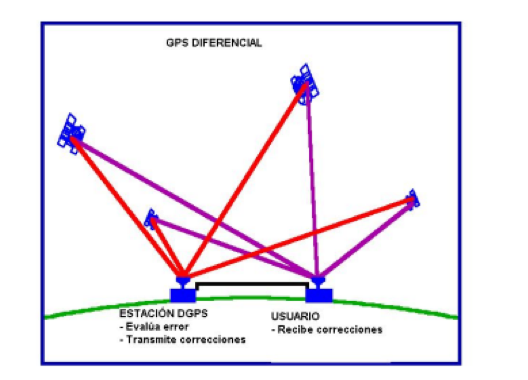
\includegraphics[width=.3\textwidth]{images/imgmarco/dgps}
		\label{fig:dgps}
	\end{center}
\end{figure}
\subsection{Estructura del DGPS}
La estructura esta de la siguiente manera:
\begin{itemize}
\item Estimación monitorizada
\item Equipo de usuario 
\item Una corrección directamente aplicada a la posición 
\item Una corrección aplicada a las pseudodistancias (Distancia media entre la antena de receptor GPS y el satélite) de cada uno de los satélites visibles.
\end{itemize}

\section{Integracion con la telefonía móvil}
Actualmente dentro del mercado de la telefonía móvil la tendencia es la de integrar, por parte de los fabricantes, la tecnología GPS dentro de sus dispositivos. El uso y masificación del GPS está particularmente extendido en los teléfonos móviles smartphone, lo que ha hecho surgir todo un ecosistema de software para este tipo de dispositivos, así como nuevos modelos de negocios que van desde el uso del terminal móvil para la navegación tradicional punto-a-punto hasta la prestación de los llamados Servicios Basados en la Localización (LBS).
Un buen ejemplo del uso del GPS en la telefonía móvil son las aplicaciones que permiten conocer la posición de amigos cercanos sobre un mapa base. Para ello basta con tener la aplicación respectiva para la plataforma deseada (Android, Bada, IOS, WP, Symbian) y permitir ser localizado por otros.

\section{Memoria Caché}
La memoria caché de un procesador, es un tipo de memoria volátil (como la memoria RAM), pero muy rápida. Su función es almacenar instrucciones y datos a los que el procesador debe acceder continuamente.\\{\bf ¿CUAL ES SU FINALIDAD?}\\Estos tipos de datos sean de acceso instantáneo para el procesador, ya que se trata de información relevante y que debe estar a la mano de manera muy fluida. Los sistemas de hardware y software llamados caché, almacenan este tipo de datos de manera duplicada y por esta razón su acceso es tan veloz.
\subsection{¿Como Funciona la memoria caché}
Cada vez que el sistema quiere acceder a un nuevo dato, éste es almacenado en la memoria caché. Entonces, cuando se necesita recurrir nuevamente al mismo dato, el sistema se dirigirá directamente al caché, haciendo así el proceso mucho más rápido. Este ciclo de almacenamiento y rescate de datos, obliga a la memoria caché a estar en continua renovación.\\Su función,es mantener de manera temporal y accesible aquellos datos que son requeridos por el sistema para realizar determinadas funciones o tareas. Así, cada vez que abras una app en tu smartphone, ésta tendrá acceso inmediato a la información que necesita para subir el nivel de eficiencia de sus funciones.
\subsection{Tipos de Memoria Caché}
Hay tres tipos de caché frecuentemente usados en computadoras personales: \\ 1.-caché de disco.\\ 2.-caché de pista.\\ 3.-caché web.\\ {\bf Caché de disco.\\}
Es una porción de memoria RAM asociada a un disco, con el fin de almacenar datos recientemente leídos y agilizar su carga en dado caso que sean solicitados otra vez. puede mejorar notablemente el rendimiento de las aplicaciones, dado que acceder a un byte de datos en RAM puede ser miles de veces más rápido que acceder a un byte del disco duro.\\
{\bf Caché de pista.\\}
Es una memoria de estado sólido tipo RAM cuyo uso de esta clase de discos generalmente se limita a las supercomputadoras por su costo tan elevado.\\
{\bf Cache web.\\}
Es la encargada de almacenar documentos web para reducir el ancho de banda consumido, la carga de los servidores y el retraso de las descargas. Existen 3 tipos de cache web: Privados que solo funcionan para un usuario, Compartidos Sirven páginas a varios usuarios y Pasarela que funcionan a cargo del propio servidor original. 
{\bf Composiciíon Interna.\\}
Los datos en la memoria caché se alojan en distintos niveles según la frecuencia de uso que tengan. La información puede transferirse entre los distintos niveles de forma inclusiva o exclusiva:\\
{\bf Caché Inclusivo.\\}
Los datos solicitados se quedan en la memoria caché de procedencia.\\
{\bf Caché Exclusivo.\\}
Los datos solicitados se eliminan de la memoria caché de procedencia una vez transferidos al nuevo nivel.\\
\subsubsection{2.8.2.1 Memoria caché nivel 1}
También llamada memoria interna, se encuentra en el núcleo del microprocesador y su capacidad es de hasta 768 kb. Es utilizada para almacenar y acceder a datos e instrucciones importantes y de uso frecuente, agilizando los procesos al ser el nivel que ofrece un tiempo de respuesta menor. Se divide en dos subniveles:\\
Nivel 1 Data Cache:\\ Se encarga de almacenar datos usados frecuentemente.\\
Nivel 1 Instruction Cache:\\ Se encarga de almacenar instrucciones usadas frecuentemente.
\subsubsection{2.8.2.2 Memoria caché nivel 2}
Se encarga de almacenar datos de uso frecuente, siendo más lenta que la caché nivel 1, pero más rápida que la memoria principal (RAM). Se encuentra en el procesador, pero no en su núcleo. Genera una copia del nivel 1.
\subsubsection{2.8.2.3 Memoria caché nivel 3}
Esta memoria genera una copia a la nivel 2. Es más rápida que la memoria principal (RAM), pero más lenta que el nivel 2. En esta memoria se agiliza el acceso a datos e instrucciones que no fueron localizadas en nivel 1 o nivel 2.\\Es generalmente de un tamaño mayor y ayuda a que el sistema guarde gran cantidad de información agilizando las tareas del procesador.\\En la actualidad esta memoria ya no es tan usada.
\section{Versiones de Android en México}
La fragmentación en Android no es un tema nuevo, aquí hemos expresado nuestra opinión más de una vez, y a pesar de que es el sistema operativo que más me gusta, cada mes queda muy claro que a Google le urge encontrar una solución para obligar o ayudar a los fabricantes a actualizar sus dispositivos.\\En el reporte de diciembre del 2017  vemos como {\bf Android Oreo} apenas está en el 0.5 porciento de todos los dispositivos del mercado, mientras que {\bf Android Nougat} que ya lleva poco más de un año alcanza ya el 23.3 porciento de cuota, sin embargo, {\bf Android 6.0 Marshmallow} tiene el 29.7 porciento y {\bf Android 5.0 Lollipop} que ya tiene más de tres años disponible está presente en el 26.3 porcirnto de smartphones con Android.
\begin{figure}[htbp]
	\begin{center}
		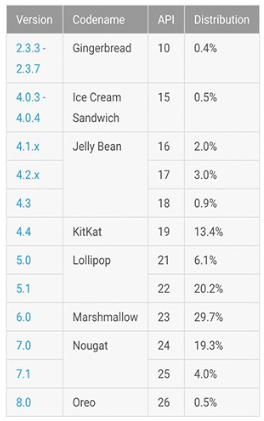
\includegraphics[width=.3\textwidth]{images/imgmarco/versiones}
		\label{fig:versiones}
	\end{center}
\end{figure}


\section{Diferencia entre GDP y DGPS}
El Sistema de Posicionamiento Global Diferencial (DGPS) es una mejora para el GPS (Sistema de Posición Global). El sistema GPS basado en la tecnología satelital puede tener una precisión nominal de 15 metros, mientras que DGPS puede alcanzar una precisión de alrededor de 10 cm. [16] DGPS usa las estaciones de referencia fijas basadas en tierra para transmitir la diferencia entre las coordenadas del GPS y la posición fija desde la estación base. La señal de corrección digital se transmite a todos los transmisores basados en tierra llamados rovers. El DGPS se basa en dos estaciones, una es la estación base y la siguiente es el usuario. 

\section{Mapas interactivos}
Los mapas interactivos que se encuentran disponibles en Internet incluyen: los geográficos, desarrollados por Google y Microsoft, los cuales proveen la funcionalidad de definir puntos de localización de puntos de interés. Sin embargo, estos mapas, en su versión satelital, tienen la limitante de que las imágenes no son actualizadas con regularidad. Por otro lado, plataformas como MapBox permite la creación de mapas interactivos. Mapbox es una plataforma que permite el desarrollo de aplicaciones móviles y aplicaciones web para la creación de mapas que permitan la localización de datos, incluyendo, además de los diseños de mapas satelitales y de calles, diseños de mapas de terrenos y tráfico [MapBox, s.f.]. MapBox ofrece un plan de costos que varía de acuerdo al número de vistas y solicitudes de información. 
En MapBox todo es 100% personalizable. Desde cualquier color hasta mostrar/ocultar capas en el mapa. Hay una serie de estilos disponibles por defecto (Dark, Light, etc.) pero también tienes la posibilidad de diseñar/crear tus propios estilos por completo a través de la herramienta Mapbox Studio. 
Todo el código está abierto y basado en estándares abiertos. Mapbox dispone de más de 500 repositorios en Github. 
No importa para qué plataforma desarrolles porque hay SDKsdisponibles para prácticamente todas. Entre las cuales están Android, iOS, Web, Qt, Unity y MacOS. Además, todas las funcionalidades están accesibles desde cada uno de ellos, ya que comparten una misma base.
Todo ocurre en tu app. No hay necesidad de tener que saltar a otra aplicación para nada (Mapbox no tiene apps para usuarios así que no tiene interés en competir con sus desarrolladores). Esto es especialmente útil si estás desarrollando una app de navegación, ya que, a diferencia de otros SDKs, puedes proveer una experiencia de navegación completa, sin perder a tus usuarios en ningún momento. Otro ejemplo es la posibilidad de guardar mapas offline sin salir de tu app.
El core está basado en mapas vectoriales implementados en C++, de forma que únicamente se mandan los datos necesarios al dispositivo y se interpretan en tiempo real, lo que se traduce en mapas muy rápidos y en visualizaciones mucho más ligeras.
Tanto el SDK de Android como el de iOS tienen una API similar a la de Google Maps y MapKit respectivamente.

\subsection{Mapas offline}
El uso de aplicaciones que puedan seguir funcionando sin conexión a internet es una característica muy importante a la hora de hablar de aplicaciones de mapeo. El poder acceder a una lista de mapas almacenados en nuestro dispositivo y eliminar los que ya no necesitemos es una opción muy atractiva para no gastar los datos de nuestro servicio de internet o en el peor caso que no tengamos red debido a que nos encontremos en un lugar sin cobertura de señal o que debido a un suceso independiente de nosotros y de nuestra compañía de servicio de internet las telecomunicaciones fallen y podamos hacer uso de esta funcionalidad sin ningún problema. 
Al poder tener esta opción de guardar regiones del mapa en nuestro dispositivo tenemos que considerar algunas cosas como que una región fuera de línea no se puede modificar después de la creación, pero es posible crear una nueva región con una definición modificada y eliminar la ya existente. Al igual una región abarca cierta dimensión, y que una vez guardada no se puede modificar, por lo que tenemos que tener en cuenta que las ubicaciones que busquemos fuera de este rango será imposible encontrarlas. Y que se tiene que considerar poder guardar en nuestro dispositivo cierta cantidad de regiones para no saturar el espacio de almacenamiento del mismo.

\section{Estado del arte}
SKY ALERT:\\CARACTERÍSTICAS\\1.-Tiene sus propios sensores de alertas sismicas.\\2.-Alerta de tormentas,Contingencias,Tsunamis y Alertas volcanicas.\\3.-Cuenta con programa de simulacro.\\4.-Cuenta con publicaciones en las redes sociales.\\5.-Requiere de una conexión a Internet.\\6.-No cuenta con repetidora de señal por estacion de radio(NOAA).\\7.-Alerta Sísmicas.\\8.- No cuenta con notificaciones push para alertas sísmicas.\\9.-No cuenta con mapeo de ruta hasta un lugar seguro.\\10.-No proporciona información de albergues.\\11.-No te deja ver mapas de albergues,refugios,centros de acopio.\\ 
\\

911 CDMX:\\CARACTERÍSTICAS\\1.-No tiene sus propios sensores de alertas sismicas.\\2.-No Alerta de tormentas,Contingencias,Tsunamis y ni de Alertas volcanicas.\\3.-No cuenta con programa de simulacro.\\4.-Cuenta con publicaciones en las redes sociales.\\5.-Requiere de una conexión a Internet.\\6.-Si cuenta con repetidora de señal por estacion de radio(NOAA).\\7.-Alerta Sísmicas.\\8.-No cuenta con notificaciones push para alertas sísmicas.\\9.-No cuenta con mapeo de ruta hasta un lugar seguro.\\10.-No proporciona información de albergues.\\11.-No te deja ver mapas de albergues,refugios,centros de acopio.\\
\\

ALERTA SÍSMICA DF:\\CARACTERÍSTICAS\\1.-No tiene sus propios sensores de alertas sismicas.\\2.-No Alerta de tormentas,Contingencias,Tsunamis y ni de Alertas volcanicas.\\3.-Cuenta con programa de simulacro.\\4.-No cuenta con publicaciones en las redes sociales.\\5.-Requiere de una conexión a Internet.\\6.-Si cuenta con repetidora de señal por estacion de radio(NOAA).\\7.-No proporciona una alerta Sísmicas.\\8.-Cuenta con notificaciones push para alertas sísmicas.\\9.-No cuenta con mapeo de ruta hasta un lugar seguro.\\10.-No proporciona información de albergues.\\11.-No te deja ver mapas de albergues,refugios,centros de acopio.\\
\\


SOLUCIÓN PROPUESTA:\\CARACTERÍSTICAS\\1.-No tiene sus propios sensores de alertas sismicas.\\2.-No Alerta de tormentas,Contingencias,Tsunamis y ni de Alertas volcanicas.\\3.-Cuenta con programa de simulacro.\\4.-No cuenta con publicaciones en las redes sociales.\\5.-No requiere de una conexión a Internet.\\6.-No cuenta con repetidora de señal por estacion de radio(NOAA).\\7.-Cuenta con Alerta Sísmicas.\\8.-Cuenta con notificaciones push para alertas sísmicas.\\9.-Cuenta con mapeo de ruta hasta un lugar seguro.\\10.-Proporciona información de albergues.\\11.-Te deja ver mapas de albergues,refugios,centros de acopio.\\
\\
DEFINICIONES:\\ \\
SKY ALERT: Es una de las herramientas con lo cual se podrá atento a cualquier movimiento telúrico y otros fenomenos naturales.\\ La plataforma tiene cobertura en la Ciudad de México, Estado de México,Puebla,Morelos,Michoacan,Guerrero,Tlaxcala,Jalisco,Colima Oaxaca  y Chiapas.\\
\\
911 CDMX: Es una aplicación para teléfonos inteligentes con sistema operativo iOS o Android, que conecta a las y los usuarios directamente al 9-1-1 de la Ciudad de México, puede ser por llamada telefónica y por chat. Además cuenta con la Alerta Sísmica, la cual se activará cuando se detecte algún sismo que por su magnitud ponga en riesgo a la CDMX.\\
\\
ALERTA SÍSMICA DF: Es una aplicación de alerta temprana que recibe notificaciones push con avisos de actividad sísmica y recibe noticias relevantes relacionadas con protección civil.\\
\\
SOLUCIÓN DE PROPUESTA: Es una aplicacion de alerta sísmica con lo cual te alertará de cualquier movimiento sísmico a tráves de notificaciones push, la aplicación tambien proporciona información de refugios ,albergues y centros de acopio ubicados en la CDMX.\\La aplicación brinda la oprtunidad de que realices tu propio registro de refugio, albergue y centro de acopio y cuenta con mapeo de ruta hasta un albergue o refugio.